\documentclass[12pt,letterpaper]{article}
\usepackage[utf8]{inputenc}
\usepackage[T1]{fontenc}
\usepackage{lmodern}
\usepackage[spanish,es-noshorthands]{babel}
\usepackage{geometry,graphicx,booktabs,array,xcolor,hyperref,parskip,fancyhdr,float,caption,longtable,enumitem,listings}
\usepackage{tikz}
\usepackage{pgfgantt}
\usetikzlibrary{shapes.geometric,positioning,arrows}
\geometry{margin=2.5cm}
\setlength{\headheight}{15pt}
\hypersetup{colorlinks=true,linkcolor=blue!50!black,urlcolor=blue!50!black,citecolor=blue!50!black,
  pdftitle={Estadio de futbol: manual de usuario y manual tecnico},
  pdfauthor={Nava Santiago Erick; Tenorio Martinez Jesus Alejandro}}
\pagestyle{fancy}
\fancyhf{}
\lhead{Estadio de fútbol --- Manual de usuario y manual técnico}
\rhead{Computación Gráfica}
\cfoot{\thepage}
\captionsetup{font=small,labelfont=bf,skip=6pt}
\setlist{itemsep=2pt,topsep=4pt}

\definecolor{azul}{RGB}{31,73,125}
\definecolor{verde}{RGB}{46,110,70}
\definecolor{naranja}{RGB}{190,105,20}
\definecolor{negro}{RGB}{40,40,40}

\lstset{
  basicstyle=\ttfamily\footnotesize,
  breaklines=true,
  columns=fullflexible,
  keepspaces=true,
  frame=single,
  rulecolor=\color{negro!40},
  backgroundcolor=\color{negro!4},
  showstringspaces=false,
  tabsize=4
}

\begin{document}
\sloppy
\hypersetup{pageanchor=false}

\begin{titlepage}
\centering
\begin{minipage}{0.42\textwidth}\centering

\includegraphics[height=3cm]{figuras/unam.png}
\end{minipage}\hfill
\begin{minipage}{0.42\textwidth}\centering

\includegraphics[height=3cm]{figuras/fi.png}
\end{minipage}

\vspace{1.2cm}
{\Large Universidad Nacional Autónoma de México\\[0.2em] Facultad de Ingeniería\par}
\vspace{0.8cm}
{\large Laboratorio de Computación Gráfica\par}
\vspace{1cm}
\rule{\textwidth}{0.8pt}\\[0.6cm]
{\LARGE\bfseries Estadio de fútbol\\[0.3em]
Recreación 3D interactiva en OpenGL\par}
\vspace{0.4cm}
{\Large Manual de usuario y manual técnico\par}
\rule{\textwidth}{0.8pt}\\[1.2cm]

\begin{tabular}{rl}
\textbf{Integrantes:} & Nava Santiago Erick\\
                      & Tenorio Martínez Jesús Alejandro\\[0.5em]
\textbf{Profesor:}    & Ing. Edén Espinoza Urzúa\\[0.5em]
\textbf{Asignatura:}  & Laboratorio de Computación Gráfica\\[0.5em]
\textbf{Semestre:}    & 2027-1\\[0.5em]
\textbf{Fecha de entrega:} & 9 de noviembre de 2026\\
\end{tabular}

\vfill
{\small Ciudad Universitaria, Ciudad de México\par}
\end{titlepage}

\hypersetup{pageanchor=true}
\pagenumbering{roman}
\tableofcontents
\clearpage

\pagenumbering{arabic}

\section*{Resumen}
\addcontentsline{toc}{section}{Resumen}
Este documento reúne el manual de usuario y el manual técnico de \emph{graficaLaboratorio}, una
recreación tridimensional de un estadio de fútbol nocturno desarrollada en C++ con OpenGL 3.3.
La escena se compone de geometría generada por código (cancha, pista atlética, gradas, fachada,
porterías, jugadores, árbitro, público, árboles, torres de iluminación, drones, ave y trofeo) y de
modelos OBJ importados con Assimp (cámaras de transmisión y autobuses de los dos equipos). Sobre
esa base se programó una secuencia de partido con máquina de estados (llegada, saque, goles,
penales y final), cinco animaciones por código y un sistema de cámaras interactivo. El manual de
usuario explica la instalación, los controles y un recorrido de demostración; el manual técnico
documenta objetivos, alcance, limitantes, metodología, arquitectura, diagrama de flujo, cronograma,
materiales y pruebas.

\part{Manual de usuario}

\section{Introducción}
El programa muestra un estadio abierto de noche, con dos equipos identificados como Pumas y
Atlante, público en las dos gradas laterales y una secuencia de partido que puede reproducirse de
forma automática o recorrerse escena por escena. El usuario puede observar la escena desde una
cámara libre, desde dos drones o desde siete vistas de transmisión, y puede activar la llegada de
los autobuses, el saque inicial, los goles, la tanda de penales, la ceremonia final y los fuegos
artificiales.

La aplicación está pensada como demostración académica: no es un videojuego, no tiene audio ni
condiciones de victoria jugables. Su propósito es exhibir el pipeline gráfico completo
(modelado, texturizado, iluminación, animación, interacción y renderizado en tiempo real).

\section{Requisitos e instalación}
\subsection{Requisitos}
\begin{itemize}
  \item Windows de 64 bits o Linux; controladores compatibles con OpenGL 3.3 Core Profile o superior.
  \item En Linux, compilador de C++ con soporte para C++11 (\texttt{g++}), GLFW 3, GLEW,
        GLM, Assimp y \texttt{pkg-config}. En Windows, usar la carpeta distribuida con el
        ejecutable y sus DLL; no se requiere compilador para ejecutarlo.
  \item Una GPU capaz de sostener la resolución del monitor a una tasa aceptable. La escena usa ocho luces
        puntuales, cuatro reflectores y sombreado por fragmento.
\end{itemize}

\subsection{Ejecución en Windows}
Descargar el repositorio y extraerlo si se obtuvo como ZIP. Abrir
\texttt{dist/graficaLaboratorio/} y hacer doble clic en
\texttt{graficaLaboratorio.exe}. Como alternativa, desde la raíz del repositorio en PowerShell:
\begin{lstlisting}
.\dist\graficaLaboratorio\graficaLaboratorio.exe
\end{lstlisting}
No separar el ejecutable de las DLL ni de las carpetas \texttt{Models/} y
\texttt{Shader/} incluidas en la misma carpeta de distribución. En Windows, el
programa establece automáticamente esa carpeta como directorio de trabajo al abrirse.

\subsection{Compilación y ejecución en Linux}
El archivo \texttt{Configinicial/build.sh} compila la biblioteca SOIL2 incluida y
genera un ejecutable nativo de Linux (no el \texttt{.exe} de Windows). En Ubuntu o
Debian, desde la raíz del repositorio, ejecutar:
\begin{lstlisting}
sudo apt update
sudo apt install build-essential pkg-config libglfw3-dev libglew-dev libglm-dev libassimp-dev
cd Configinicial
./build.sh
./graficaLaboratorio
\end{lstlisting}
En ejecuciones posteriores basta con entrar en \texttt{Configinicial/} y ejecutar
\texttt{./graficaLaboratorio}. Debe iniciarse desde esa carpeta porque los shaders,
las texturas y los modelos se buscan mediante rutas relativas (\texttt{Shader/},
\texttt{Models/}); desde otra ubicación pueden faltar recursos.

\section{Controles}
La ventana abre a la resolución del monitor y el título muestra el marcador, el tiempo, la escena
actual, el estado de pausa y los penales. La proyección se ajusta al tamaño del framebuffer cuando
la ventana cambia. La tabla~\ref{tab:controles} resume todas las teclas implementadas
en \texttt{main.cpp}.

\begin{longtable}{p{0.16\textwidth}p{0.50\textwidth}p{0.26\textwidth}}
\caption{Controles del programa.}\label{tab:controles}\\
\toprule
\textbf{Tecla} & \textbf{Acción} & \textbf{Contexto}\\
\midrule
\endfirsthead
\toprule
\textbf{Tecla} & \textbf{Acción} & \textbf{Contexto}\\
\midrule
\endhead
\bottomrule
\endfoot
\texttt{Esc} & Cierra la ventana. & Siempre\\
\texttt{0} & Activa la cámara libre y reinicia la orientación del ratón. & Siempre\\
Ratón & Gira la cámara libre (yaw y pitch). & Cámara 0\\
\texttt{W}/\texttt{S} & Avanza o retrocede. & Cámara 0\\
\texttt{A}/\texttt{D} o $\leftarrow$/$\rightarrow$ & Se desplaza a la izquierda o a la derecha. & Cámara 0\\
\texttt{1}, \texttt{2} & Selecciona el dron 1 o el dron 2. & Siempre\\
\texttt{W}/\texttt{S}/\texttt{A}/\texttt{D} & Desplaza el dron en el plano horizontal. & Drones 1--2\\
\texttt{Q}/\texttt{E} & Baja o sube el dron. & Drones 1--2\\
\texttt{Shift} & Duplica la velocidad del dron. & Drones 1--2\\
\texttt{3}--\texttt{8} & Selecciona una cámara fija de transmisión; el cabezal sigue al balón. & Siempre\\
\texttt{9} & Vista aérea cenital; en la final apunta al trofeo. & Siempre\\
\texttt{Z} & Inicia la llegada de los autobuses. & Desde el estado inicial\\
\texttt{L} & Reinicia y reproduce la secuencia completa automática. & Siempre\\
\texttt{Espacio} & Desde el estado inicial reproduce toda la secuencia automáticamente (llegada, saque, dos goles, penales y final); durante la secuencia la pausa o reanuda. & Siempre\\
\texttt{X} & Salta al saque inicial. & Siempre\\
\texttt{C} & Salta al gol de Pumas. & Siempre\\
\texttt{V} & Salta al gol de Atlante. & Siempre\\
\texttt{N} & Salta a la tanda de penales. & Siempre\\
\texttt{P} & Ejecuta un tiro penal. & Escena de penales\\
\texttt{M} & Salta a la final con fuegos artificiales. & Siempre\\
\texttt{F} & Lanza fuegos artificiales desde cualquier escena. & Siempre\\
\texttt{R} & Reinicia el partido y vuelve al estado inicial. & Siempre\\
\texttt{H} & Enciende o apaga los faros de los autobuses. & Siempre\\
$\uparrow$/$\downarrow$ & Aumenta o reduce la intensidad de las cuatro torres. & Siempre\\
\texttt{[}/\texttt{]} & Gira 90$^\circ$ los modelos de cámara de transmisión. & Siempre\\
\end{longtable}

\section{Secuencia del partido}
El programa implementa seis escenas además del estado inicial. Cada cambio se hace con una
transición de fundido; la tabla~\ref{tab:escenas} describe qué ocurre en cada una.

\begin{table}[H]
\centering
\small
\begin{tabular}{p{0.17\textwidth}p{0.18\textwidth}p{0.53\textwidth}}
\toprule
\textbf{Escena} & \textbf{Tecla} & \textbf{Contenido}\\
\midrule
Inicial & \texttt{R} & Estadio nocturno, público en las gradas, trofeo en el pedestal y drones en vuelo.\\
Llegada & \texttt{Z} & Los dos autobuses entran por los accesos, giran, se detienen y los jugadores bajan y forman.\\
Saque & \texttt{X} & Balón al centro; el jugador 10 de Atlante ejecuta el saque y el balón avanza por el campo.\\
Gol de Pumas & \texttt{C} & Tiro de esquina, dos remates de cabeza y gol; el público de Pumas festeja y el rival reacciona.\\
Gol de Atlante & \texttt{V} & Jugada de Atlante, remate y gol; se invierte el festejo.\\
Penales & \texttt{N} & Tanda con portero animado, marcador de penales y reacciones según el resultado.\\
Final & \texttt{M} & El capitán levanta el trofeo, el público celebra y se lanzan fuegos artificiales.\\
\bottomrule
\end{tabular}
\caption{Escenas y teclas de acceso.}\label{tab:escenas}
\end{table}

Para reproducir el partido completo, desde el estado inicial pulse \texttt{Espacio}: el programa
inicia automáticamente la llegada de los autobuses, el saque, el gol de Pumas, el gol de Atlante,
la tanda de penales y la ceremonia final con fuegos artificiales. Durante el recorrido, otra
pulsación de \texttt{Espacio} pausa la secuencia y la siguiente la reanuda; no la reinicia.
\texttt{L} sí reinicia y reproduce la secuencia completa desde cualquier escena. En los penales
automáticos el programa dispara cada intento y decide al ganador. Si se entra con \texttt{N}, la
secuencia no es automática y cada tiro debe ordenarse con \texttt{P}; esto permite explicar la
animación paso a paso.

\begin{figure}[H]
\centering
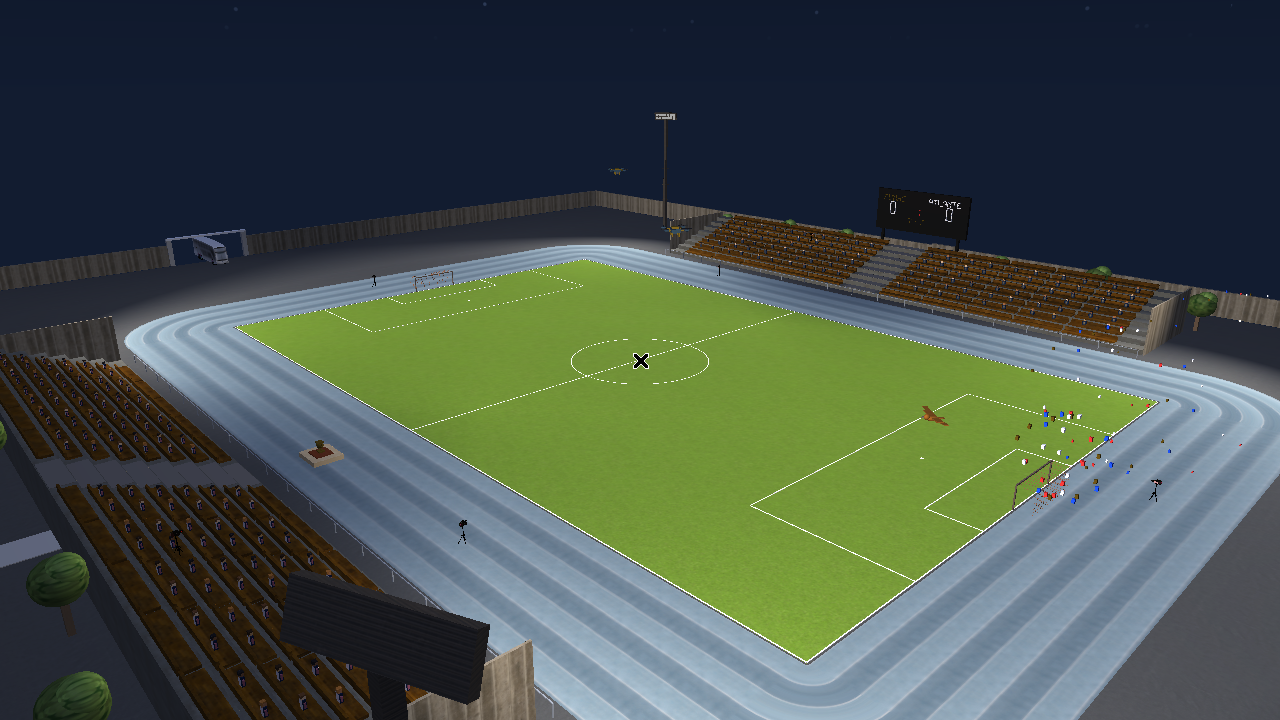
\includegraphics[width=0.88\textwidth]{figuras/estadio_general.png}
\caption{Vista general del estadio desde la cámara libre: cancha, pista atlética, gradas, fachada y torres de iluminación.}
\label{fig:general}
\end{figure}

\begin{figure}[H]
\centering
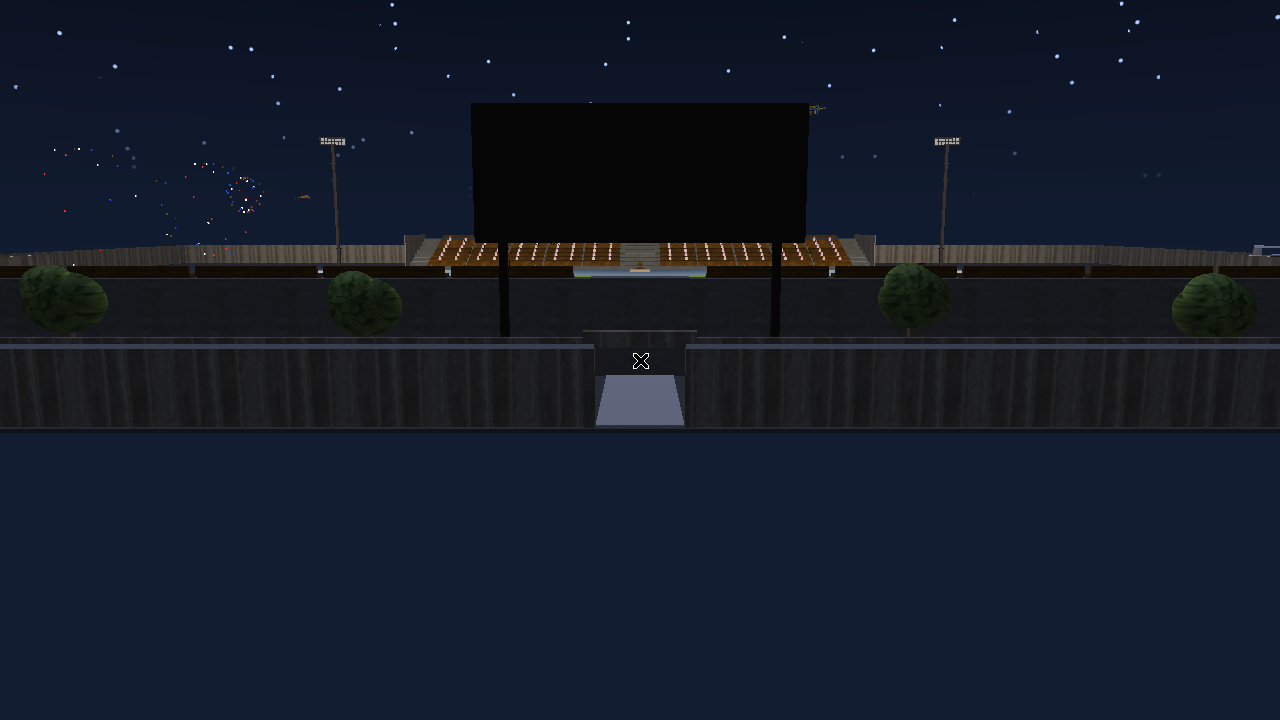
\includegraphics[width=0.88\textwidth]{figuras/fachada.png}
\caption{Fachada perimetral y accesos vistos desde el exterior. La llegada de los autobuses usa estos accesos.}
\label{fig:fachada}
\end{figure}

\section{Recorrido recomendado para la demostración}
El siguiente recorrido cubre los requisitos de la entrega en menos de cinco minutos:
\begin{enumerate}
  \item Iniciar el programa y observar la vista aérea con \texttt{9}. Comentar la planta del
        estadio, la pista y las cuatro torres.
  \item Pulsar \texttt{0} y recorrer la fachada con \texttt{W}/\texttt{A}/\texttt{S}/\texttt{D} y el
        ratón (figura~\ref{fig:fachada}).
  \item Volver a una vista fija con \texttt{5} y pulsar \texttt{Z} para la llegada. Encender los
        faros con \texttt{H} (figura~\ref{fig:autobuses}).
  \item Pulsar \texttt{R} y después \texttt{Espacio} para reproducir la secuencia completa desde el inicio. Dejar que se vean el saque, los dos
        goles y el festejo del público (figuras~\ref{fig:publico} y~\ref{fig:arbitro}).
  \item En los penales, si se desea control manual, pulsar \texttt{N} y luego \texttt{P} para cada
        tiro (figura~\ref{fig:penal}).
  \item Pulsar \texttt{M} para la final y los fuegos (figuras~\ref{fig:trofeo} y~\ref{fig:fuegos}).
  \item Cerrar con \texttt{Esc}.
\end{enumerate}

\section{Solución de problemas}
\begin{itemize}
  \item \textbf{La ventana no abre o se cierra de inmediato.} Verificar que el equipo tenga
        controladores OpenGL 3.3 y que el ejecutable se lance desde \texttt{Configinicial/}.
  \item \textbf{Aparecen mensajes \texttt{Texture not loaded} o \texttt{Missing team bus}.} Faltan
        archivos de \texttt{Models/}. Revisar que la carpeta completa se haya copiado y que las
        rutas conserven mayúsculas y minúsculas.
  \item \textbf{Algunos objetos se ven de color plano.} Es el respaldo previsto cuando una textura no
        se encuentra; el programa sigue funcionando con \texttt{CreateSolidColorTexture}.
  \item \textbf{Rendimiento bajo.} La escena dibuja cientos de cubos y carga modelos OBJ pesados.
        Cerrar otras aplicaciones y usar una resolución de ventana menor ayuda; la geometría no se
        simplifica en tiempo de ejecución.
  \item \textbf{Los penales no avanzan solos.} Si se entró con \texttt{N}, hay que pulsar \texttt{P}
        en cada intento. La secuencia automática solo se activa con \texttt{L} o \texttt{Espacio}.
\end{itemize}

\begin{figure}[H]
\centering
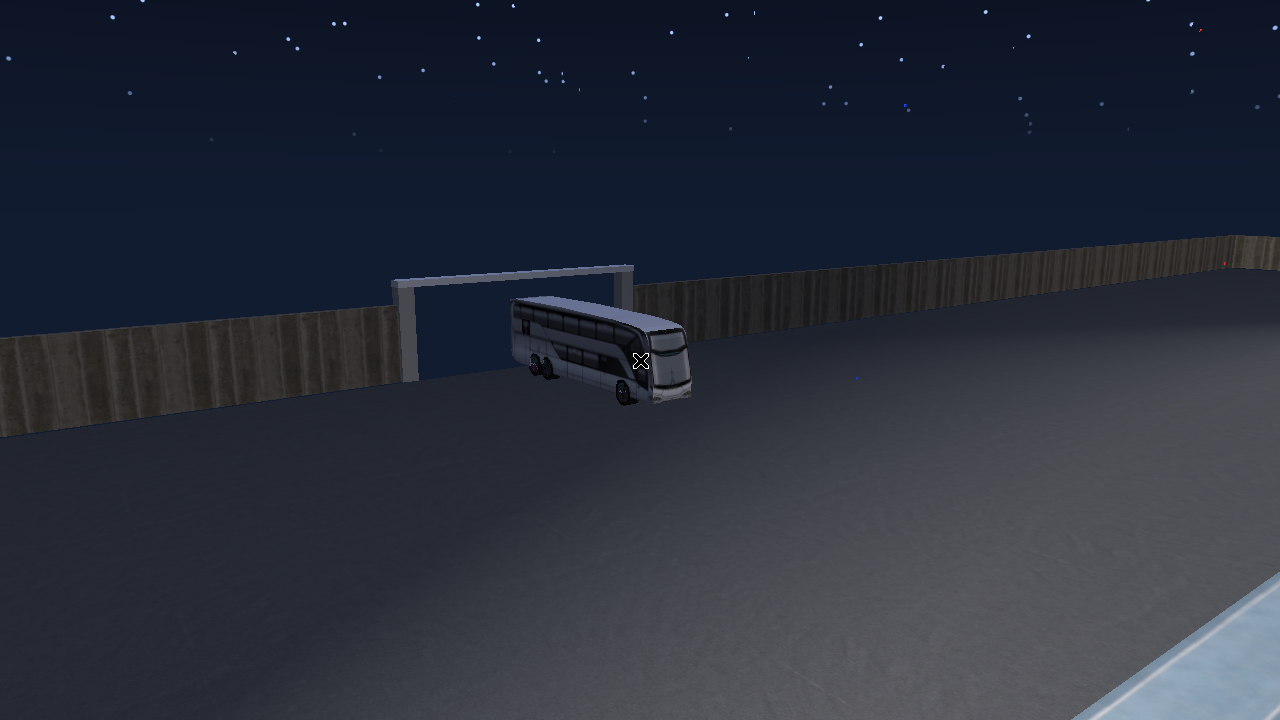
\includegraphics[width=0.88\textwidth]{figuras/autobuses.png}
\caption{Llegada de un autobús por el acceso lateral, con faros encendidos.}
\label{fig:autobuses}
\end{figure}

\begin{figure}[H]
\centering
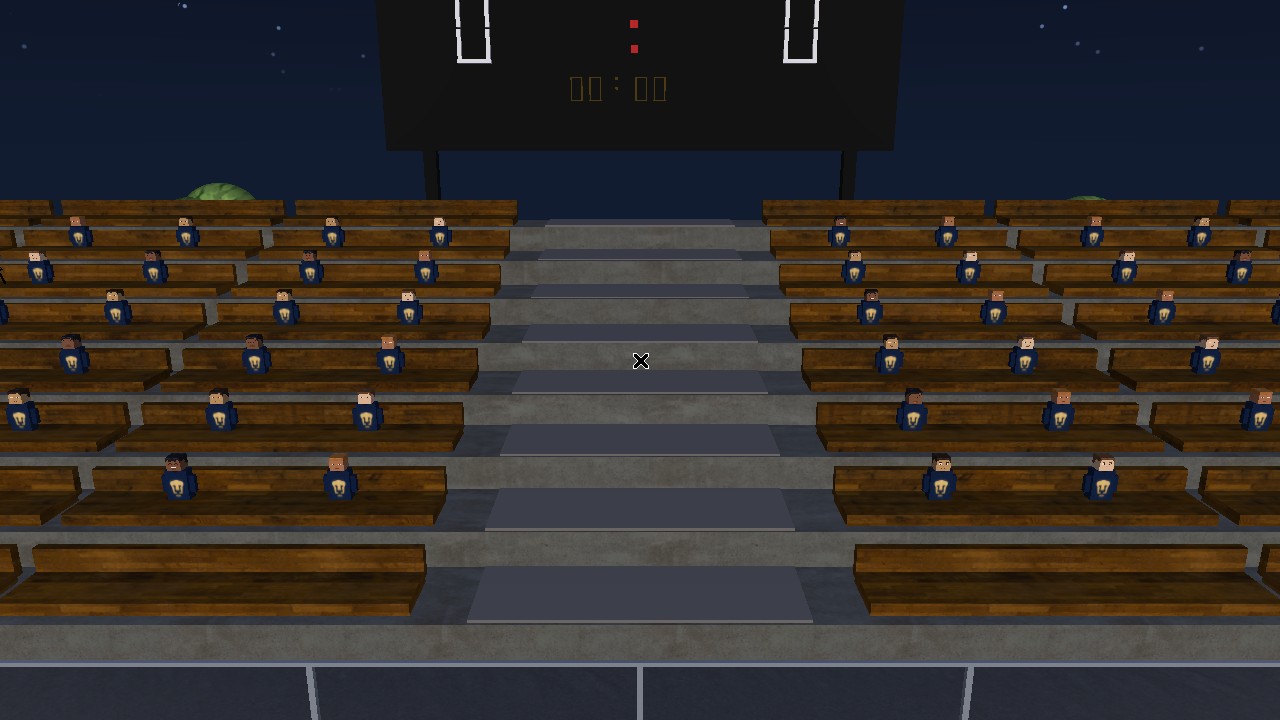
\includegraphics[width=0.88\textwidth]{figuras/publico.png}
\caption{Público en la grada de Pumas: playeras, rostros diferenciados y butacas de madera.}
\label{fig:publico}
\end{figure}

\begin{figure}[H]
\centering
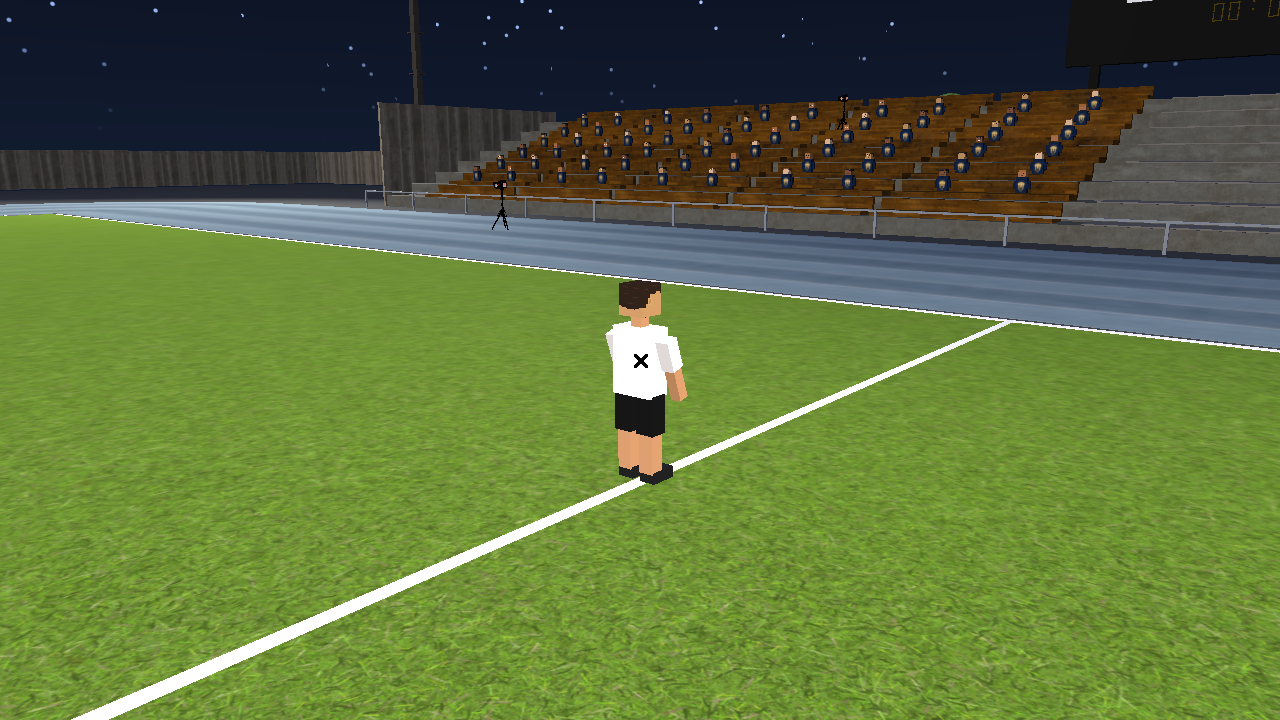
\includegraphics[width=0.80\textwidth]{figuras/arbitro.png}
\caption{Árbitro con playera amarilla texturizada durante el saque inicial.}
\label{fig:arbitro}
\end{figure}

\begin{figure}[H]
\centering
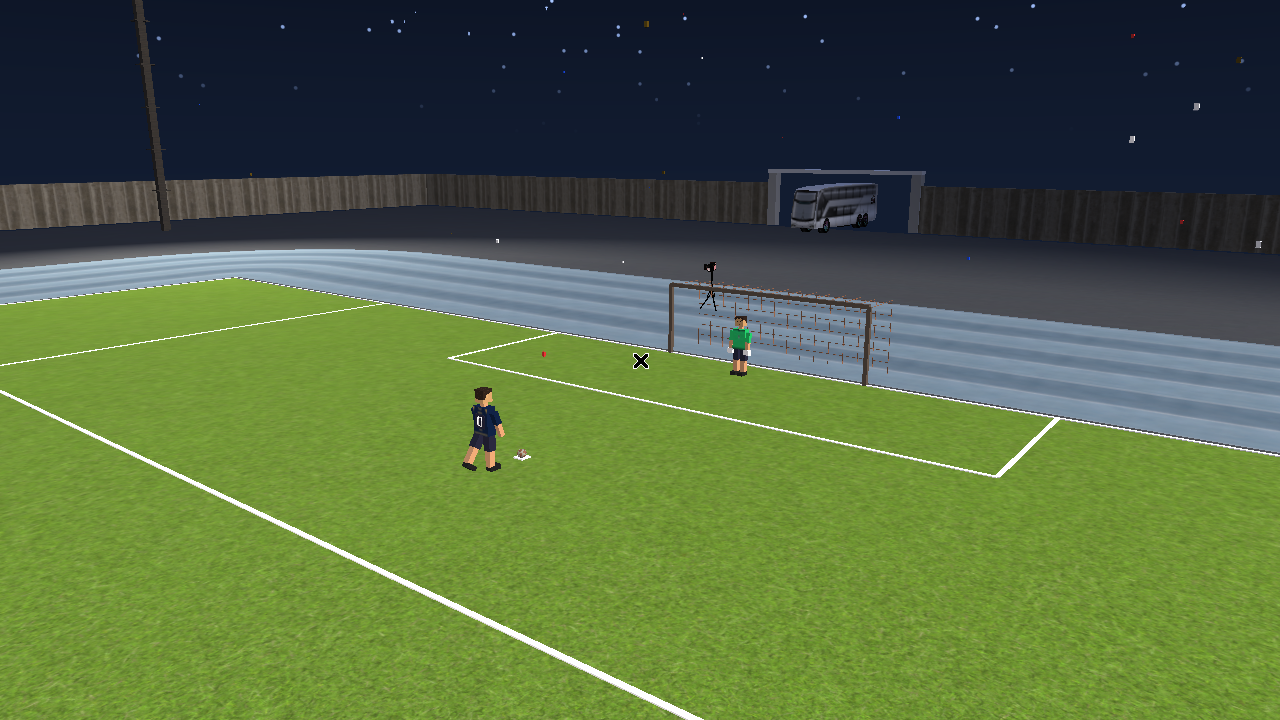
\includegraphics[width=0.88\textwidth]{figuras/penal.png}
\caption{Tiro penal: balón, portero y portería con red texturizada.}
\label{fig:penal}
\end{figure}

\begin{figure}[H]
\centering
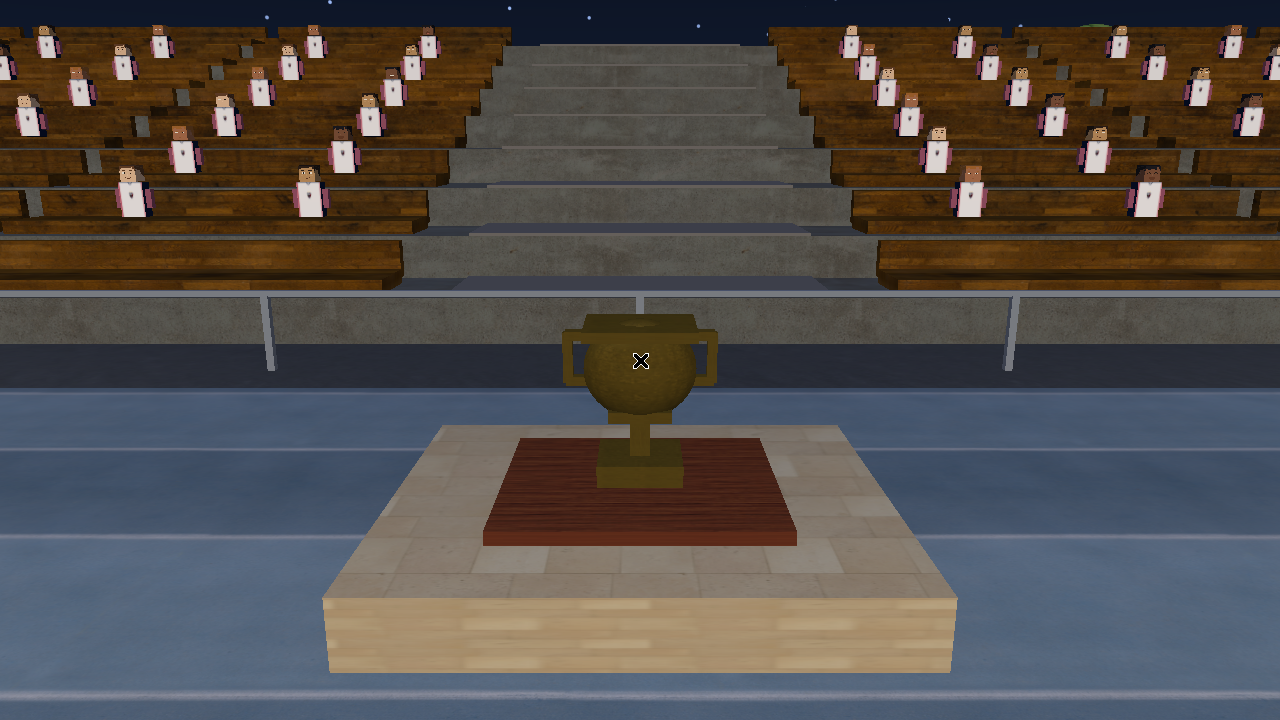
\includegraphics[width=0.88\textwidth]{figuras/trofeo.png}
\caption{Trofeo sobre su pedestal, con mapas de oro, mármol y madera.}
\label{fig:trofeo}
\end{figure}

\begin{figure}[H]
\centering
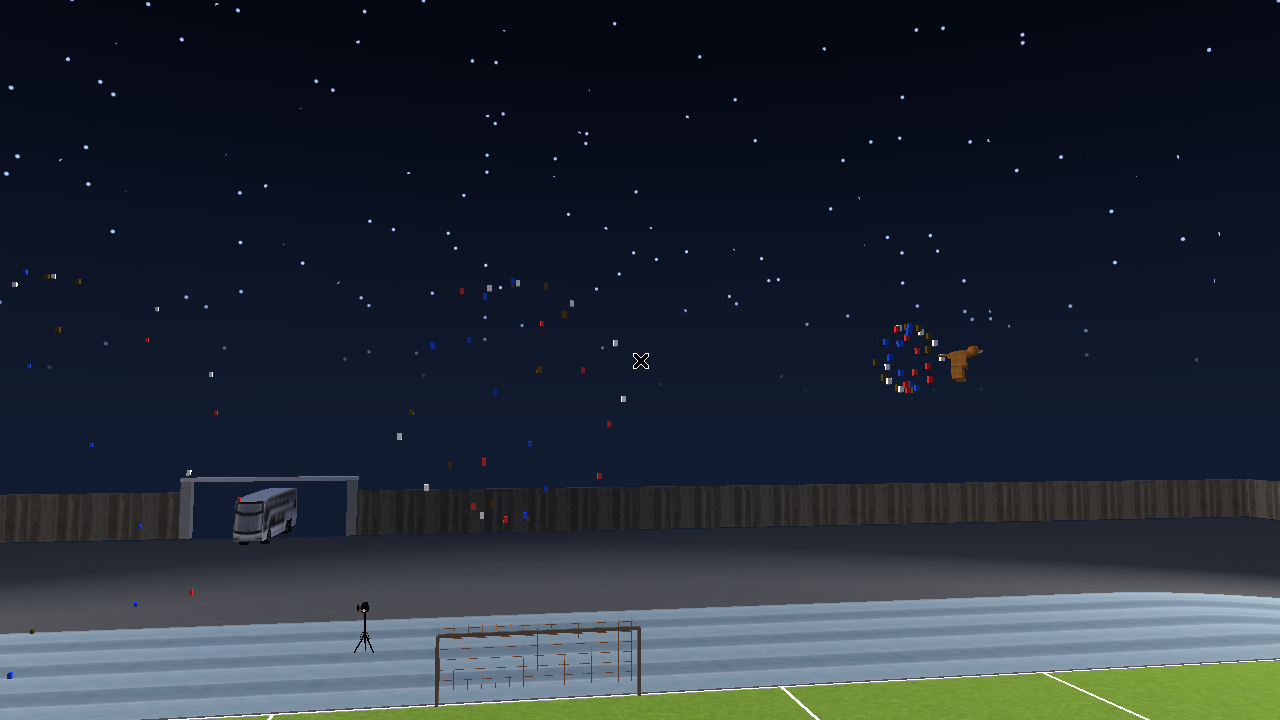
\includegraphics[width=0.88\textwidth]{figuras/fuegos.png}
\caption{Fuegos artificiales calculados por código durante la ceremonia final.}
\label{fig:fuegos}
\end{figure}

\clearpage
\part{Manual técnico}

\section{Objetivos}
\subsection{Objetivo general}
Aplicar los conocimientos del curso de Computación Gráfica para construir, documentar y exponer una
recreación tridimensional interactiva de un estadio de fútbol, usando OpenGL 3.3, geometría generada
por código, modelos importados, texturizado, iluminación, animación por estados e interacción en
tiempo real.

\subsection{Objetivos específicos}
\begin{itemize}
  \item Recrear una fachada y un espacio con al menos siete tipos de objetos distintos, con geometría
        y texturizado adecuados.
  \item Conservar y extender la base docente de las prácticas (contexto OpenGL, cámara, shaders,
        carga de modelos, texturizado, iluminación y máquinas de estados).
  \item Programar al menos cinco animaciones: tres sencillas y dos complejas.
  \item Implementar una secuencia de partido coherente con el tema, con transiciones y estados.
  \item Documentar el uso del programa, la arquitectura, el flujo, el cronograma, el alcance, las
        limitantes y las pruebas.
\end{itemize}

\section{Alcance}
El sistema cubre una cancha de fútbol con pista atlética, gradas laterales, fachada perimetral con
dos accesos, cuatro torres de iluminación, árboles, porterías, marcador, dos equipos de once
jugadores, árbitro, público, cámaras de transmisión, dos drones, un ave, un trofeo y dos autobuses
importados. La interacción se limita a recorrer la escena, cambiar de cámara, controlar la secuencia
y ajustar la iluminación; no hay edición de la escena, audio, colisiones ni modo multijugador.

La tabla~\ref{tab:objetos} enumera los tipos de objeto con texturizado de imagen. Los objetos
repetidos (jugadores, butacas, árboles, torres) cuentan como un solo tipo, y los detalles de
ambientación no se usan para completar el mínimo de siete.

\begin{table}[H]
\centering
\small
\begin{tabular}{p{0.26\textwidth}p{0.62\textwidth}}
\toprule
\textbf{Tipo de objeto} & \textbf{Texturas principales}\\
\midrule
Cancha & \texttt{Grass005\_Color}\\
Pista atlética & \texttt{running\_track\_diff\_1k}\\
Gradas y butacas & \texttt{gravel\_concrete\_03}, \texttt{old\_wooden\_floor\_02}\\
Fachada y accesos & \texttt{concrete\_diff\_1k}, \texttt{worn\_shutter\_diff\_1k}\\
Porterías & \texttt{metal\_plate\_02}, \texttt{fabric\_leather\_01}\\
Balón & \texttt{leather\_white}, \texttt{fabric\_leather\_01}\\
Jugadores & Playeras PNG, atlas de rostro, shorts y piel planos\\
Árbitro & \texttt{referee\_yellow\_jersey}, atlas de rostro\\
Público & Playeras PNG y cuatro atlas de rostro\\
Árboles & \texttt{pine\_bark}, \texttt{LeafSet024\_Dark/Light}\\
Torres de iluminación & \texttt{worn\_shutter\_diff\_1k}\\
Cámaras de transmisión & Modelos OBJ con logo Liga MX\\
Autobuses & Carrocerías y ruedas OBJ con sus mapas\\
Drones & \texttt{blue\_metal\_plate}, \texttt{metal\_plate\_04}, \texttt{rubber\_tiles}\\
Ave & \texttt{fabric\_leather\_02}, \texttt{rough\_wood}\\
Trofeo & \texttt{trophy\_gold}, \texttt{marble\_01}, \texttt{dark\_wood}\\
\bottomrule
\end{tabular}
\caption{Tipos de objeto y texturas asociadas.}\label{tab:objetos}
\end{table}

\section{Limitantes}
\begin{itemize}
  \item \textbf{Texturizado procedural.} La geometría creada con cubos y esferas no tiene UV
        modelados a mano. El sombreador calcula coordenadas a partir de la posición o la normal, de
        modo que en algunas caras el mapa se estira o se repite. Los uniformes, la piel, el calzado y
        varios accesorios siguen usando color plano.
  \item \textbf{Cámaras fijas.} Las cámaras 3--8 apuntan siempre al balón y no permiten encuadres
        libres. La cámara 9 es una vista cenital, no una vista de fachada; para observar la fachada
        se usa la cámara libre. La redistribución de cámaras propuesta en la rama \texttt{camaras}
        no está integrada.
  \item \textbf{Sin sombras proyectadas.} La iluminación es local (Phong/Blinn-Phong); no hay mapas
        de sombra ni oclusión ambiental.
  \item \textbf{Sin audio ni físicas.} No hay sonido, colisiones, rebotes reales ni simulación de
        multitudes.
  \item \textbf{Dependencia de rutas relativas.} El ejecutable debe correr desde \texttt{Configinicial/}.
  \item \textbf{Plataforma.} La compilación reproducible documentada es Linux mediante
        \texttt{build.sh}; el proyecto de Visual Studio existe, pero no se validó en esta entrega.
  \item \textbf{Repetición de geometría.} El público y los jugadores se dibujan con cubos y esferas
        reutilizados; no son mallas esculpidas.
\end{itemize}

\section{Metodología de software aplicada}
Se siguió un desarrollo incremental con control de versiones Git y ramas por aportación:
\begin{enumerate}
  \item \textbf{Análisis de la consigna y diseño.} Lectura de los requisitos, definición de la
        planta del estadio y del conjunto de escenas.
  \item \textbf{Base gráfica.} Contexto OpenGL 3.3, ventana GLFW, entrada, cámara, shaders de
        iluminación y carga de modelos con Assimp.
  \item \textbf{Modelado por código.} Cancha, pista, gradas, fachada, porterías, jugadores, árbitro,
        público, árboles, torres, drones, ave y trofeo.
  \item \textbf{Texturizado e iluminación.} Mapas de color CC0, atlas de rostros, playeras generadas
        por script y luces puntuales y reflectores.
  \item \textbf{Animación y estados.} Llegada de autobuses, saque, goles, penales, final, festejos y
        fuegos artificiales.
  \item \textbf{Verificación.} Compilación con \texttt{build.sh} y quince scripts de comprobación en
        \texttt{Configinicial/tests/}.
  \item \textbf{Documentación.} Este manual y el archivo de pendientes.
\end{enumerate}
El historial de Git se usó como registro real de avances: primer commit el 28 de octubre de 2026,
base avanzada el 5 de noviembre, texturas y escena el 7 y 8 de noviembre, y animaciones finales el
9 de noviembre. Los commits se agruparon por ramas de trabajo (\texttt{erick-jisus},
\texttt{rama-chui}, \texttt{camaras}, \texttt{limpieza-repo}) y se integraron en \texttt{main}.

\section{Arquitectura del software}
\subsection{Archivos y responsabilidades}
\begin{table}[H]
\centering
\small
\begin{tabular}{p{0.30\textwidth}p{0.58\textwidth}}
\toprule
\textbf{Archivo o carpeta} & \textbf{Responsabilidad}\\
\midrule
\texttt{main.cpp} & Inicialización, recursos, bucle, entrada, escenas, animaciones y dibujo.\\
\texttt{Camera.h} & Cámara con vectores front/up/right y ángulos de Euler (base docente).\\
\texttt{Shader.h} & Compilación, enlace y activación de programas GLSL (base docente).\\
\texttt{Model.h}, \texttt{Mesh.h} & Carga y dibujo de mallas OBJ con Assimp (base docente).\\
\texttt{Shader/lighting.*} & Iluminación Phong/Blinn-Phong, ocho luces puntuales y cuatro reflectores.\\
\texttt{Shader/sky.*} & Cielo nocturno procedural con estrellas y luna.\\
\texttt{Shader/lamp.*} & Dibujo de las lámparas de las torres.\\
\texttt{Models/} & Modelos OBJ, mapas de color, playeras y atlas de rostros.\\
\texttt{SOIL2/} & Carga de imágenes a texturas OpenGL.\\
\texttt{tests/} & Quince comprobaciones de código, texturas y geometría.\\
\texttt{build.sh} & Compilación reproducible en Linux.\\
\bottomrule
\end{tabular}
\caption{Organización del proyecto.}\label{tab:archivos}
\end{table}

\subsection{Bucle principal}
El programa usa tres programas GLSL: \texttt{lightingShader} para la escena,
\texttt{lampShader} para las lámparas y \texttt{skyShader} para el fondo. En cada cuadro se leen los
eventos, se actualiza el tiempo y, si la secuencia no está pausada, se ejecutan el movimiento de
cámara o dron, la lógica de la escena, la animación del penal y la de los autobuses. Después se
configuran cámara y luces, se dibuja el cielo sin escritura de profundidad, se dibuja la escena con
profundidad y se intercambian los búferes.

\begin{lstlisting}
glfwPollEvents();
if (!sequencePaused) {
    animationClock += deltaTime;
    DoMovement();
    updateMatch(deltaTime);
    if (matchScene == SCENE_PENALTIES && fadePhase != FADE_OUT) Animation();
    if (matchScene == SCENE_ARRIVAL && fadePhase != FADE_OUT) updateBusAnimation();
    updateFade(deltaTime);
}
view = getBroadcastView();
projection = glm::perspective(glm::radians(fov), aspect, 0.1f, 300.0f);
\end{lstlisting}

\section{Diagrama de flujo del software}
La figura~\ref{fig:flujo} muestra el flujo por cuadro. La decisión de pausa omite las actualizaciones
pero mantiene el dibujo, de modo que la ventana sigue respondiendo. La decisión de escena activa
controla la máquina de estados del partido; el estado inicial solo dibuja la escena y el trofeo.

\begin{figure}[H]
\centering
\begin{tikzpicture}[
  node distance=5mm,
  box/.style={draw=azul!70, fill=azul!8, rounded corners=2pt, text width=5.2cm,
              align=center, minimum height=8mm, font=\small},
  dec/.style={draw=naranja!80!black, fill=naranja!15, diamond, aspect=2.4,
              text width=3.1cm, align=center, inner sep=1pt, font=\small},
  io/.style={draw=verde!60!black, fill=verde!10, rounded corners=6pt,
             text width=4.6cm, align=center, minimum height=8mm, font=\small},
  arr/.style={-latex, thick, draw=negro!75}
]
\node[io] (ini) {Inicio};
\node[box, below=of ini] (init) {Inicializar GLFW/GLEW, compilar shaders, cargar texturas y modelos OBJ};
\node[box, below=of init] (loop) {Bucle: \texttt{glfwPollEvents}, \texttt{deltaTime}, entrada};
\node[dec, below=of loop] (pause) {¿Secuencia pausada?};
\node[box, below=of pause] (upd) {\texttt{DoMovement}, \texttt{updateMatch}, \texttt{Animation}, \texttt{updateBusAnimation}, \texttt{updateFade}};
\node[box, below=of upd] (draw) {Configurar cámara y luces; dibujar cielo, escena y HUD};
\node[box, below=of draw] (swap) {\texttt{glfwSwapBuffers}};
\draw[arr] (ini) -- (init);
\draw[arr] (init) -- (loop);
\draw[arr] (loop) -- (pause);
\draw[arr] (pause) -- node[right,font=\scriptsize]{no} (upd);
\draw[arr] (upd) -- (draw);
\draw[arr] (draw) -- (swap);
\draw[arr] (pause.east) -- ++(2.4,0) |- node[pos=0.25,right,font=\scriptsize]{sí} (draw.east);
\draw[arr] (swap.west) -- ++(-3.4,0) |- (loop.west);
\end{tikzpicture}
\caption{Diagrama de flujo del programa. El ciclo se repite hasta que se cierra la ventana.}
\label{fig:flujo}
\end{figure}

\section{Diagrama de Gantt}
El cronograma de la figura~\ref{fig:gantt} usa las fechas reales del historial de Git. La escala
comienza el 28 de octubre de 2026 y termina el 9 de noviembre, fecha de entrega.

\begin{figure}[H]
\centering
\begin{ganttchart}[
  hgrid, vgrid,
  x unit=0.66cm,
  y unit chart=0.62cm,
  bar height=0.48,
  bar/.append style={fill=azul!55, draw=azul!85!black},
  milestone/.append style={fill=naranja!85, draw=naranja!60!black},
  title/.append style={draw=none, fill=none},
  title label font=\scriptsize,
  bar label font=\scriptsize,
  milestone label font=\scriptsize,
  bar label node/.append style={text width=3.5cm, align=right}
]{1}{13}
\gantttitle{Octubre}{4}\gantttitle{Noviembre}{9}\\
\gantttitlelist{28,29,30,31}{1}\gantttitlelist{1,...,9}{1}\\
\ganttbar{Análisis y diseño inicial}{1}{4}\\
\ganttbar{Geometría del estadio}{1}{9}\\
\ganttbar{Cámara, shaders y luces}{5}{9}\\
\ganttbar{Texturas y materiales}{10}{12}\\
\ganttbar{Modelos OBJ importados}{11}{11}\\
\ganttbar{Público y árbitro}{12}{12}\\
\ganttbar{Animaciones y secuencia}{11}{13}\\
\ganttbar{Pruebas y documentación}{12}{13}\\
\ganttmilestone{Entrega}{13}
\end{ganttchart}
\caption{Cronograma del proyecto con fechas del historial de Git.}
\label{fig:gantt}
\end{figure}

\begin{table}[H]
\centering
\small
\begin{tabular}{p{0.46\textwidth}p{0.22\textwidth}p{0.22\textwidth}}
\toprule
\textbf{Actividad} & \textbf{Periodo} & \textbf{Responsable}\\
\midrule
Análisis de la consigna y diseño inicial & 28--31 oct & Erick Nava\\
Geometría del estadio y la cancha & 28 oct--5 nov & Erick Nava\\
Cámara, shaders e iluminación & 1--5 nov & Erick Nava\\
Texturas y materiales & 6--8 nov & Jesús Tenorio\\
Modelos OBJ de cámaras y autobuses & 7 nov & Erick Nava\\
Público, árbitro y reacciones & 8 nov & Jesús Tenorio\\
Animaciones y secuencia de partido & 7--9 nov & Ambos\\
Pruebas, documentación y entrega & 8--9 nov & Ambos\\
\bottomrule
\end{tabular}
\caption{Actividades, periodos y responsables.}\label{tab:gantt}
\end{table}

\section{Documentación del código}
\subsection{Estados del partido}
La máquina de estados principal usa la enumeración \texttt{MatchScene}. La tabla~\ref{tab:estados}
resume las transiciones automáticas y manuales.

\begin{table}[H]
\centering
\small
\begin{tabular}{p{0.21\textwidth}p{0.27\textwidth}p{0.42\textwidth}}
\toprule
\textbf{Estado} & \textbf{Contenido} & \textbf{Salida}\\
\midrule
\texttt{SCENE\_IDLE} & Estadio, trofeo y drones. & \texttt{Z}, \texttt{L}, \texttt{Espacio} o salto directo.\\
\texttt{SCENE\_ARRIVAL} & Autobuses y formación. & Automática al completar la formación; o \texttt{X}.\\
\texttt{SCENE\_KICKOFF} & Saque y desplazamiento del balón. & Automática a los 6.2 s; o \texttt{C}.\\
\texttt{SCENE\_PUMAS\_GOAL} & Jugada, remates y festejo. & Automática a los 8.3 s; o \texttt{V}.\\
\texttt{SCENE\_ATLANTE\_GOAL} & Jugada y festejo visitante. & Automática a los 6.5 s; o \texttt{N}.\\
\texttt{SCENE\_PENALTIES} & Tanda, portero y marcador. & Automática al decidir ganador; o \texttt{M}.\\
\texttt{SCENE\_FINAL} & Trofeo, celebración y fuegos. & \texttt{R} para reiniciar.\\
\bottomrule
\end{tabular}
\caption{Estados de la secuencia de partido.}\label{tab:estados}
\end{table}

Cada cambio pasa por \texttt{requestMatchScene}: si la escena actual es el estado inicial se cambia
de inmediato; en otro caso se activa \texttt{FADE\_OUT}, se dibuja un velo negro y, al llegar a
opacidad total, \texttt{beginMatchScene} reinicia el tiempo y entra con \texttt{FADE\_IN}. La variable
\texttt{autoSequence} decide si las escenas se encadenan solas o esperan una tecla.

\subsection{Tiro penal}
El penal usa la enumeración \texttt{PenaltyState}: \texttt{READY}, \texttt{PREPARING},
\texttt{KICKING}, \texttt{FLYING} y \texttt{FINISHED}. En \texttt{PREPARING} el tirador retrocede;
en \texttt{KICKING} se aplica el ángulo de patada y el portero elige lado; en \texttt{FLYING} el
balón interpola hacia un objetivo aleatorio dentro de la portería y el portero extiende el cuerpo;
en \texttt{FINISHED} se registra gol o atajada, se actualizan los marcadores y se decide el ganador
cuando la ventaja es matemáticamente irreversible. El límite de intentos por equipo es 64.

\subsection{Llegada de autobuses}
Cada autobús recorre una recta de 28 unidades y después un arco de 90$^\circ$ con radio 8 hasta
quedar alineado con la cancha. La posición y el giro se calculan con \texttt{distanceTraveled},
\texttt{busSpeed} y \texttt{busTurnRadius}; las ruedas giran según la velocidad y el volante. Al
detenerse, los once jugadores de cada equipo bajan con un retardo de 0.62 s y caminan 3.7 s hasta
su formación. Los faros se encienden con \texttt{H} y la animación se activa con \texttt{Z},
\texttt{L} o \texttt{Espacio}.

\subsection{Funciones de dibujo}
\begin{table}[H]
\centering
\small
\begin{tabular}{p{0.34\textwidth}p{0.54\textwidth}}
\toprule
\textbf{Función} & \textbf{Propósito}\\
\midrule
\texttt{drawField} & Césped, líneas y áreas de la cancha.\\
\texttt{drawRunningTrack} & Pista atlética perimetral con esquinas redondeadas.\\
\texttt{drawPerimeter} & Muros, fachada, piso exterior y accesos.\\
\texttt{drawGoal} & Postes y red de las dos porterías.\\
\texttt{drawBleachers} & Gradas, butacas y pasillos.\\
\texttt{drawPlayer} & Jugador articulado con playera, cabeza, shorts, piel y calzado.\\
\texttt{drawGoalkeeperSave} & Portero con estirada y guantes.\\
\texttt{drawCelebrationCaptain} & Capitán que levanta el trofeo.\\
\texttt{drawCrowd} & 120 aficionados por grada con cuatro rostros y festejo.\\
\texttt{drawTrees} & Troncos y copas con mapas de corteza y hojas.\\
\texttt{drawDrone} & Dron con cuatro rotores giratorios y lente.\\
\texttt{drawBird} & Ave que orbita y aletea.\\
\texttt{drawTrophy} & Trofeo con base, copa y asas.\\
\texttt{drawFireworks} & Tres estallidos de partículas calculadas.\\
\texttt{drawMatchScoreboard} & Marcador 3D con dígitos de siete segmentos.\\
\texttt{drawBroadcastCameraModels} & Cámaras OBJ con cabezal que sigue al balón.\\
\texttt{drawFloodlightTowers} & Cuatro torres con paneles de iluminación.\\
\texttt{updateMatch} & Máquina de estados y trayectorias del balón.\\
\texttt{Animation} & Máquina de estados del penal.\\
\texttt{updateBusAnimation} & Ruta, ruedas y descenso de jugadores.\\
\bottomrule
\end{tabular}
\caption{Funciones principales de dibujo y actualización.}\label{tab:funciones}
\end{table}

\subsection{Sistema de cámaras}
La cámara libre usa \texttt{Camera} (base docente) con posición, yaw y pitch; se mueve con
\texttt{W}/\texttt{A}/\texttt{S}/\texttt{D} y se orienta con el ratón. Los drones 1 y 2 se desplazan
con las mismas teclas, \texttt{Q}/\texttt{E} y \texttt{Shift}; sus posiciones se limitan a
$x\in[-64,64]$, $y\in[7,34]$ y $z\in[-47,47]$. Las cámaras 3--8 son modelos OBJ colocados en
posiciones fijas; su cabezal calcula yaw y pitch hacia \texttt{trackedBallPosition}, que se suaviza
con una interpolación exponencial. La cámara 9 es cenital y en la final apunta al trofeo.

\subsection{Iluminación y cielo}
\texttt{Shader/lighting.frag} implementa el modelo de Phong/Blinn-Phong con luz ambiental, difusa y
especular, ocho luces puntuales y cuatro reflectores. Las cuatro torres aportan los reflectores; las
flechas arriba/abajo escalan su intensidad entre 0.15 y 2.5 sin afectar los faros de los autobuses.
\texttt{Shader/sky.frag} reconstruye la dirección del rayo con la inversa de la proyección y de la
rotación de la vista, genera un degradado nocturno, estrellas por \emph{hashing} de celdas y una luna
con sombra. El cielo se dibuja primero, sin prueba de profundidad, para que no tape la escena.

\subsection{Texturizado procedural}
La geometría por código no tiene coordenadas UV explícitas. El sombreador de vértices
\texttt{Shader/lighting.vs} selecciona un modo con el uniforme \texttt{proceduralTextureMode} y
calcula \texttt{TexCoords} a partir de la posición o la normal. La tabla~\ref{tab:modos} describe los
modos usados.

\begin{table}[H]
\centering
\small
\begin{tabular}{p{0.09\textwidth}p{0.24\textwidth}p{0.55\textwidth}}
\toprule
\textbf{Modo} & \textbf{Uso} & \textbf{Coordenadas}\\
\midrule
0 & UV explícitos & Atributo \texttt{texCoords} (modelos importados y caras con UV).\\
1 & Cancha & \texttt{(x,z)} escalado 12$\times$8.\\
2 & Muros & Proyección lateral y altura.\\
3 & Fachada y paneles & \texttt{(x,y)} centrado.\\
4 & Piso exterior & \texttt{(x,z)} escalado 20$\times$16.\\
5 & Gradas & Triplanar en coordenadas de mundo, escala 1/4.\\
6 & Esferas & Longitud y latitud de la normal, cuatro repeticiones.\\
7 & Cajas & Triplanar de posición local, escala 2.\\
\bottomrule
\end{tabular}
\caption{Modos de texturizado procedural.}\label{tab:modos}
\end{table}

\begin{lstlisting}
if (proceduralTextureMode == 1)
    TexCoords = (position.xz + vec2(0.5)) * vec2(12.0, 8.0);
else if (proceduralTextureMode == 5)
    TexCoords = (abs(normal.y) > 0.5 ? FragPos.xz :
                 vec2(abs(normal.x) > 0.5 ? FragPos.z : FragPos.x, FragPos.y)) / 4.0;
else if (proceduralTextureMode == 6)
    TexCoords = vec2(atan(normal.z, normal.x) * 0.1591549 + 0.5,
                     asin(clamp(normal.y, -1.0, 1.0)) * 0.3183098 + 0.5) * 4.0;
else
    TexCoords = texCoords;
\end{lstlisting}

\subsection{Modelos importados y recursos}
Se importan dos carrocerías de autobús, seis ruedas y dos piezas de cámara de transmisión
(\texttt{cameraBase.obj} y \texttt{cameraHead.obj}). \texttt{VerifyModelTextures} revisa que las
rutas declaradas en los MTL existan antes de cargar. El modelo más pesado de \texttt{Models/} mide
aproximadamente 69 MB, por debajo del límite de 100 MB por modelo. Las texturas de color provienen de
ambientCG y Poly Haven con licencia CC0; las playeras, los rostros y el logo se generan o adaptan en
el proyecto.

\subsection{Uso del código base del profesor}
El proyecto parte de la base docente de las prácticas P1--P10 y la conserva como esqueleto:
\begin{itemize}
  \item \textbf{P1:} inicialización de GLFW/GLEW, contexto OpenGL 3.3, doble búfer y callbacks.
  \item \textbf{P2--P3:} pipeline de transformaciones con GLM, \texttt{Shader.h} y VAO/VBO del cubo.
  \item \textbf{P4:} modelado jerárquico para las extremidades de jugadores y árbitro.
  \item \textbf{P5 y P8:} carga de modelos con Assimp (\texttt{Model.h}, \texttt{Mesh.h}).
  \item \textbf{P6:} texturizado con SOIL2, UV y atlas.
  \item \textbf{P7--P8:} cámara, iluminación Phong/Blinn-Phong y shaders \texttt{lighting}/\texttt{lamp}.
  \item \textbf{P9--P10:} interpolación temporal y máquinas de estados para las animaciones.
\end{itemize}
La base se extendió con el cielo procedural, los modos de textura, el público, el árbitro, las
reacciones, los autobuses y la secuencia de partido. Los archivos de la base que el proyecto usa
directamente son \texttt{Camera.h}, \texttt{Shader.h}, \texttt{Model.h}, \texttt{Mesh.h} y los shaders
de iluminación y lámpara.

\subsection{Pruebas}
La carpeta \texttt{Configinicial/tests/} contiene quince scripts de verificación. No usan un marco de
pruebas unitarias: leen el código o las imágenes y fallan con una aserción cuando falta un recurso,
una ruta o una propiedad geométrica.

\begin{table}[H]
\centering
\small
\begin{tabular}{p{0.46\textwidth}p{0.42\textwidth}}
\toprule
\textbf{Script} & \textbf{Qué comprueba}\\
\midrule
\texttt{check\_ball\_and\_goalkeeper\_textures.py} & Texturas del balón y playera distinta del portero.\\
\texttt{check\_ball\_visibility.py} & El balón aparece en juego y no en llegada o festejos.\\
\texttt{check\_camera\_logo.py} & Ruta y UV del logo Liga MX en la cámara.\\
\texttt{check\_crowd\_celebration.py} & Solo festeja la grada que anota o gana.\\
\texttt{check\_crowd.py} & Playeras y rostros distintos en ambas gradas.\\
\texttt{check\_drone\_and\_bird\_textures.py} & Mapas PBR de drones y ave.\\
\texttt{check\_goal\_textures.py} & Texturas de postes y red con mapeo triplanar.\\
\texttt{check\_night\_sky.py} & El cielo sigue a la vista sin tapar el estadio.\\
\texttt{check\_player\_head.py} & Atlas de rostro generado sin escribir en recursos.\\
\texttt{check\_pumas\_goal\_contact.py} & Contacto del balón en córner, remates y tiro.\\
\texttt{check\_referee.py} & Playera reproducible y un árbitro por escena.\\
\texttt{check\_rival\_goal\_emotions.py} & Emociones del rival al recibir gol.\\
\texttt{check\_running\_track.py} & Pista alineada a los cuatro lados sin cubrir la cancha.\\
\texttt{check\_stadium\_materials.py} & Mapas de gradas y butacas; atenuación de torres.\\
\texttt{check\_trophy\_textures.py} & Oro, mármol y madera del trofeo.\\
\bottomrule
\end{tabular}
\caption{Scripts de verificación.}\label{tab:pruebas}
\end{table}

\section{Modelos y escena}
La figura~\ref{fig:modelos} reúne los modelos que no forman parte de la arquitectura del estadio:
la cámara de transmisión importada, un dron, el ave, el trofeo, el árbitro y un autobús. Las
figuras~\ref{fig:camara} a~\ref{fig:ave} muestran cada uno por separado.

\begin{figure}[H]
\centering
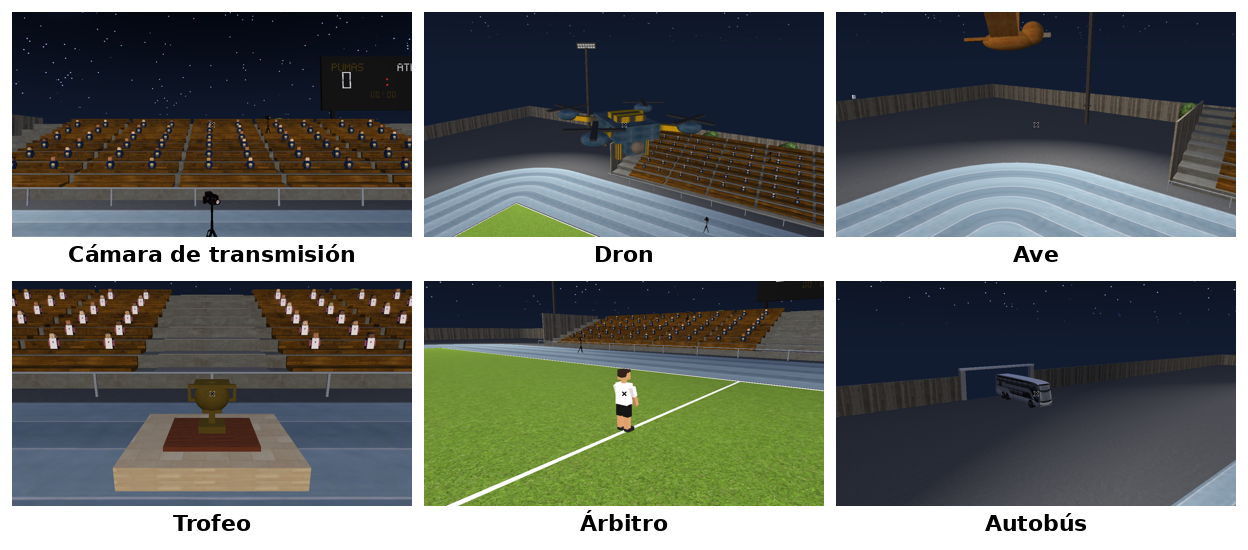
\includegraphics[width=0.95\textwidth]{figuras/modelos.png}
\caption{Lámina de modelos: cámara OBJ, dron, ave, trofeo, árbitro y autobús.}
\label{fig:modelos}
\end{figure}

\begin{figure}[H]
\centering
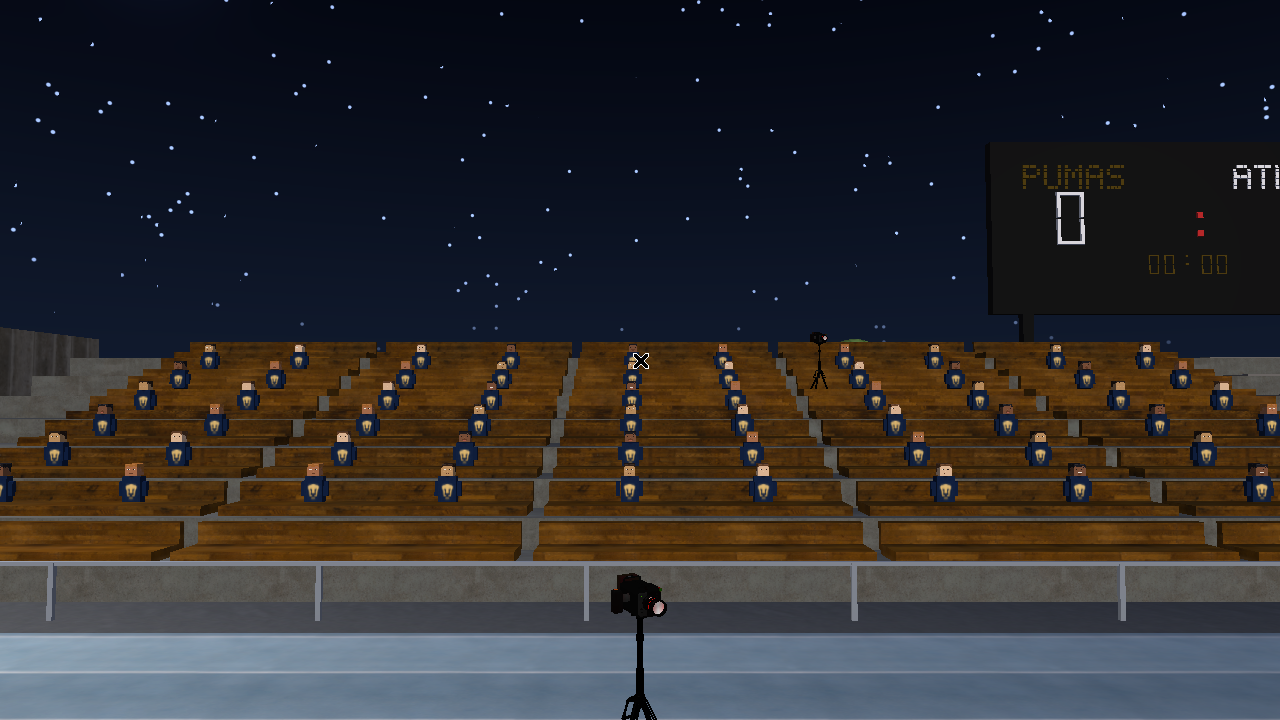
\includegraphics[width=0.82\textwidth]{figuras/camara.png}
\caption{Cámara de transmisión importada con Assimp; el cabezal apunta al balón.}
\label{fig:camara}
\end{figure}

\begin{figure}[H]
\centering
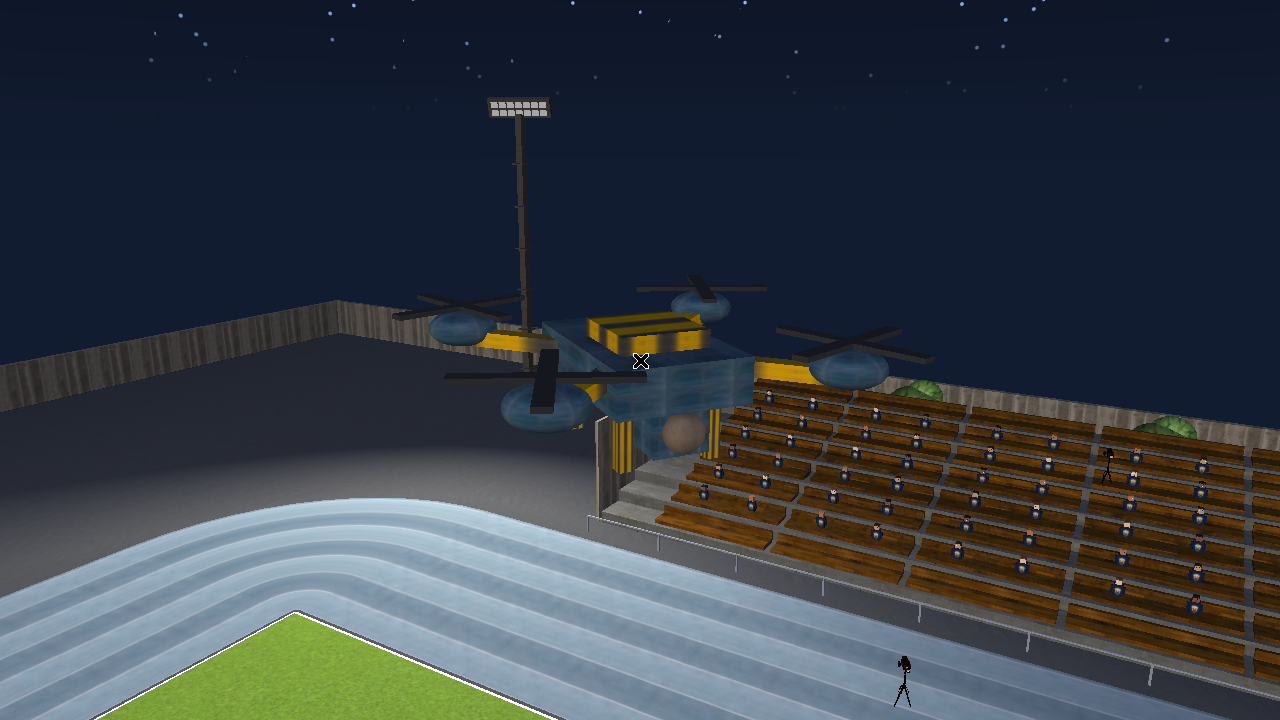
\includegraphics[width=0.82\textwidth]{figuras/dron.png}
\caption{Dron de vigilancia con rotores animados y lente metálica.}
\label{fig:dron}
\end{figure}

\begin{figure}[H]
\centering
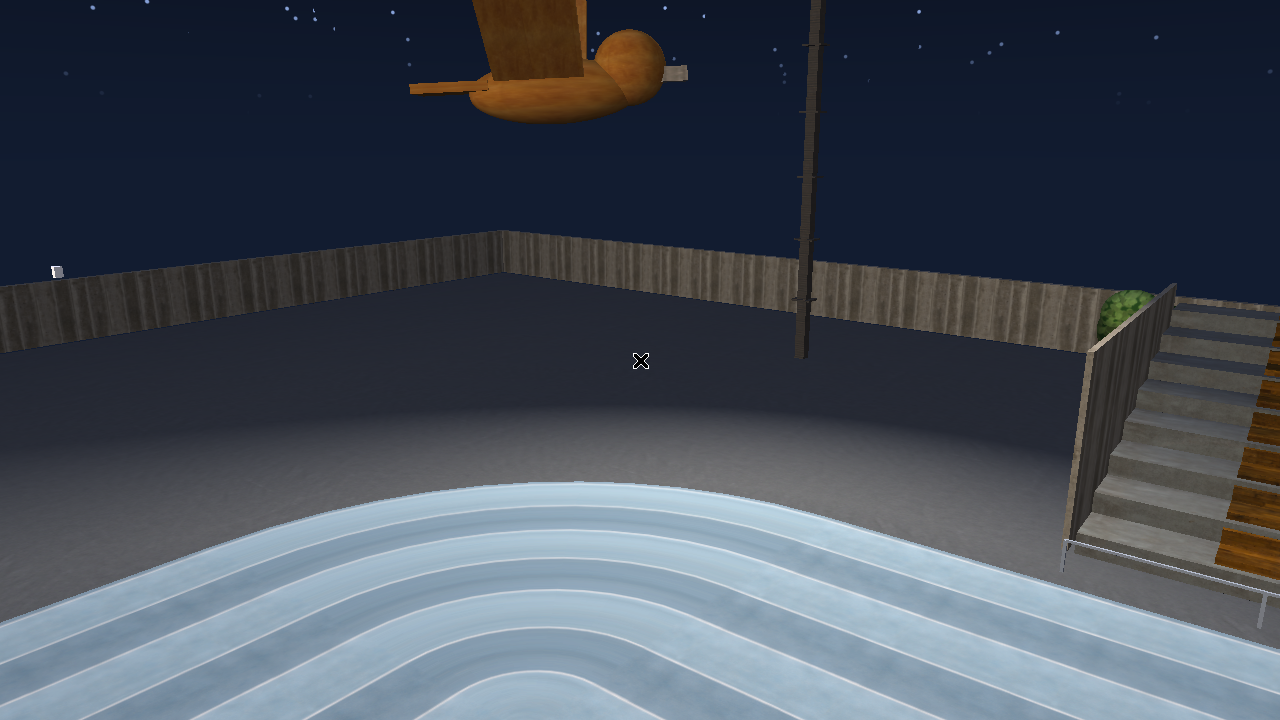
\includegraphics[width=0.82\textwidth]{figuras/ave.png}
\caption{Ave en órbita sobre el estadio; el aleteo se calcula con funciones seno.}
\label{fig:ave}
\end{figure}

\begin{figure}[H]
\centering
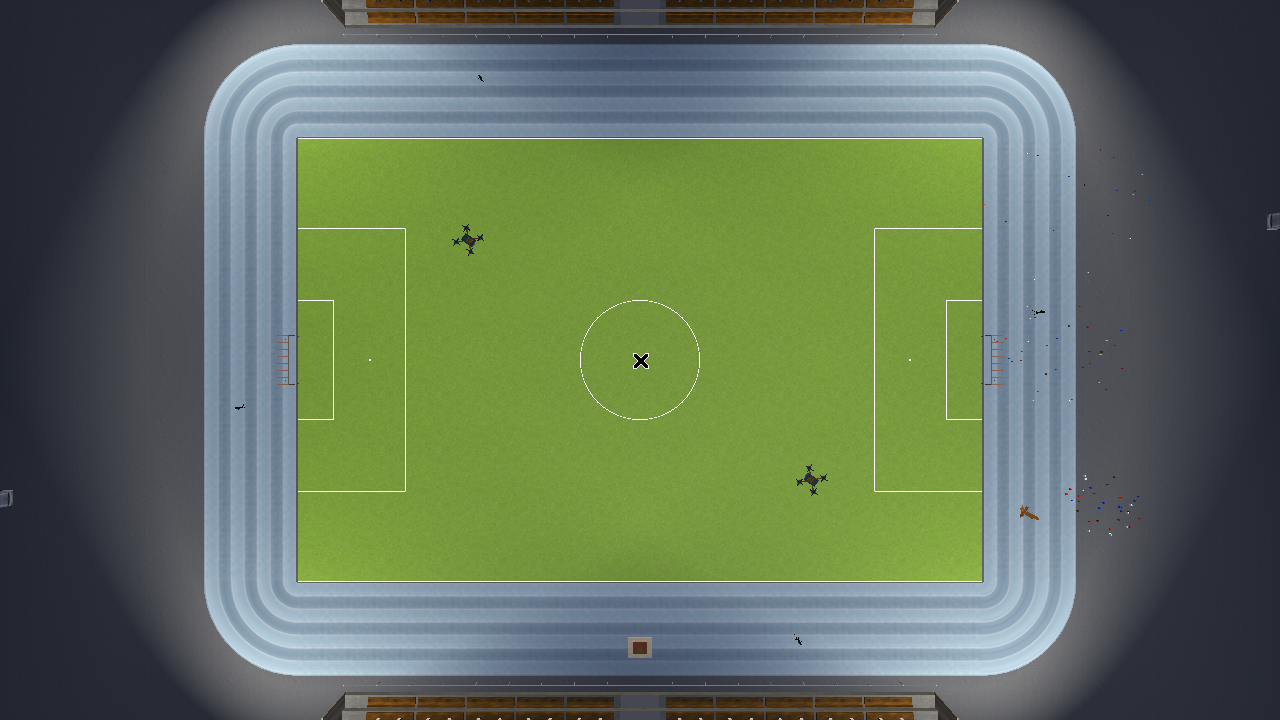
\includegraphics[width=0.88\textwidth]{figuras/vista_aerea.png}
\caption{Vista cenital de la cámara 9: planta del estadio, pista y distribución de las gradas.}
\label{fig:aerea}
\end{figure}

\section{Materiales y texturas}
La figura~\ref{fig:texturas} presenta una selección de los mapas de color usados en la escena. Los
mapas de ambientCG y Poly Haven son CC0; las playeras de Pumas, Atlante, portero y árbitro, así como
los atlas de rostro, se generan con los scripts de \texttt{Models/Textures/}. El logo de Liga MX se
aplica al cabezal de la cámara de transmisión.

\begin{figure}[H]
\centering
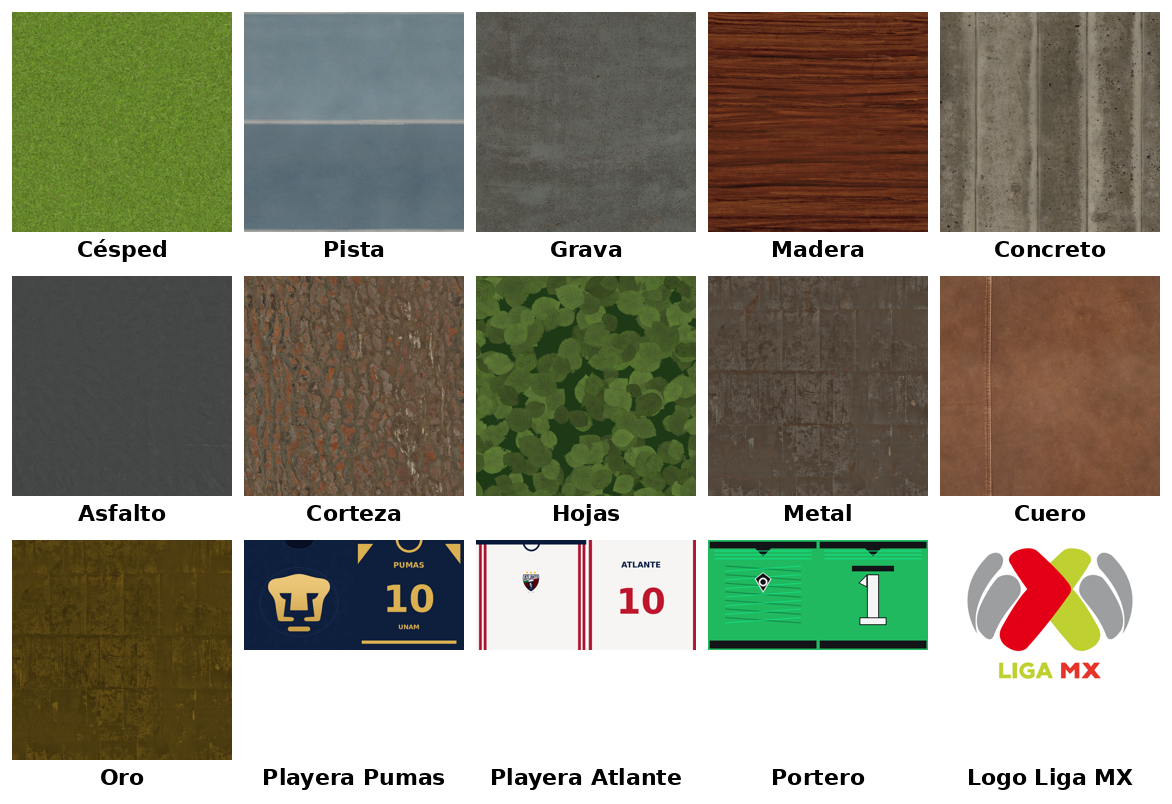
\includegraphics[width=0.98\textwidth]{figuras/texturas.png}
\caption{Lámina de texturas: césped, pista, grava, madera, concreto, asfalto, corteza, hojas, metal, cuero, oro, playeras y logo.}
\label{fig:texturas}
\end{figure}

El sombreador recibe dos unidades de textura: el mapa difuso en la unidad 0 y un mapa especular
compartido en la unidad 1. Los modelos importados usan sus propios materiales y UV; la geometría
por código usa los modos procedurales de la tabla~\ref{tab:modos}. Cuando una imagen no se
encuentra, \texttt{LoadDiffuseTexture} devuelve 0 y el programa usa
\texttt{CreateSolidColorTexture} para no dejar la cara sin material.

\end{document}
